\documentclass[12t,letterpaper]{article}

\newenvironment{proof}{\noindent{\bf Proof:}}{\qed\bigskip}

\newtheorem{theorem}{Theorem}
\newtheorem{corollary}{Corollary}
\newtheorem{lemma}{Lemma} 
\newtheorem{claim}{Claim}
\newtheorem{fact}{Fact}
\newtheorem{definition}{Definition}
\newtheorem{assumption}{Assumption}
\newtheorem{observation}{Observation}
\newtheorem{example}{Example}
\newcommand{\qed}{\rule{7pt}{7pt}}

\newcommand{\assignment}[4]{
\thispagestyle{plain} 
\newpage
\setcounter{page}{1}
\noindent
\begin{center}
\framebox{ \vbox{ \hbox to 6.28in
{\bf EE 126: Probability and Random Processes \hfill #1}
\vspace{4mm}
\hbox to 6.28in
{\hspace{2.5in}\large\mbox{#2}}
\vspace{4mm}
\hbox to 6.28in
{{\it Handed Out: #3 \hfill Due: #4}}
}}
\end{center}
}

\newcommand{\solution}[3]{
\thispagestyle{plain} 
\newpage
\setcounter{page}{1}
\noindent
\begin{center}
\framebox{ \vbox{ \hbox to 6.28in
{\bf EE 126 \hfill #3}
\vspace{4mm}
\hbox to 6.28in
{\hspace{2.5in}\large\mbox{#2}}
\vspace{4mm}
\hbox to 6.28in
{#1 \hfill}
}}
\end{center}
\markright{#1}
}

\newenvironment{algorithm}
{\begin{center}
\begin{tabular}{|l|}
\hline
\begin{minipage}{1in}
\begin{tabbing}
\quad\=\qquad\=\qquad\=\qquad\=\qquad\=\qquad\=\qquad\=\kill}
{\end{tabbing}
\end{minipage} \\
\hline
\end{tabular}
\end{center}}

\def\Comment#1{\textsf{\textsl{$\langle\!\langle$#1\/$\rangle\!\rangle$}}}


\usepackage{amsmath, dsfont, mathtools, verbatim, tikz, float}

\usetikzlibrary{arrows,automata}

\oddsidemargin 0in
\evensidemargin 0in
\textwidth 6.5in
\topmargin -0.5in
\textheight 9.0in

\newenvironment{amatrix}[1]{%
  \left(\begin{array}{@{}*{#1}{c}|c@{}}
}{%
  \end{array}\right)
}

\DeclarePairedDelimiter{\ceil}{\lceil}{\rceil}
\DeclareMathOperator*{\argmin}{arg\,min}
\DeclareMathOperator*{\argmax}{arg\,max}

\makeatletter
\renewcommand*\env@matrix[1][*\c@MaxMatrixCols c]{%
  \hskip -\arraycolsep
  \let\@ifnextchar\new@ifnextchar
  \array{#1}}
\makeatother

\newcommand{\norm}[1]{\left\lVert #1 \right\rVert}
\newcommand{\abs}[1]{\left\vert #1 \right\vert}
\newcommand{\?}{\stackrel{?}{=}}
\newcommand\given[1][]{\:#1\vert\:}
\renewcommand{\d}[1]{\ensuremath{\operatorname{d}\!{#1}}}

\begin{document}

\solution{Nikhil Unni}{HW9}{Spring 2016}
\pagestyle{myheadings}

\begin{enumerate}
  \item Midterm
    \begin{enumerate}
      \item [1.]
        \begin{enumerate}
          \item [(a)]
            \begin{enumerate}
              \item [(1)]
                False, we just don't have a unique distribution
              \item [(2)]
                False, but the converse is true
              \item [(3)]
                False, the sum of exponential distributions is the Erlang distribution
            \end{enumerate}

          \item [(b)]
            Taking derivatives of the MGF, we have:
            $$M_X(0) = a_0 = 1$$
            $$M_x'(0) = 2a_2(0) + a_1 = E[X]$$
            $$M_x''(0) = 2a_2 = E[X^2]$$
            Since Var = $E[X]$, we know that:
            $$a_1 = 2a_2 - a_1^2$$
            Solving, we get $a_0 = a_1 = a_2 = 1$.

          \item [(c)]
            Probability to decode 3 after 3rd transmission is the same as the probability of sending 3 of the same in an XOR message. Concretely, this is:
            $$\text{P(1st chunk is in 2nd transmission)P(2nd chunk is in 3rd transmission)}$$
            $$=\frac{1}{5} * 3(\frac{1}{5} \frac{1}{4})$$
            $$=\frac{3}{50}$$

          \item [(d)]
            \begin{enumerate}
              \item [(i)]
                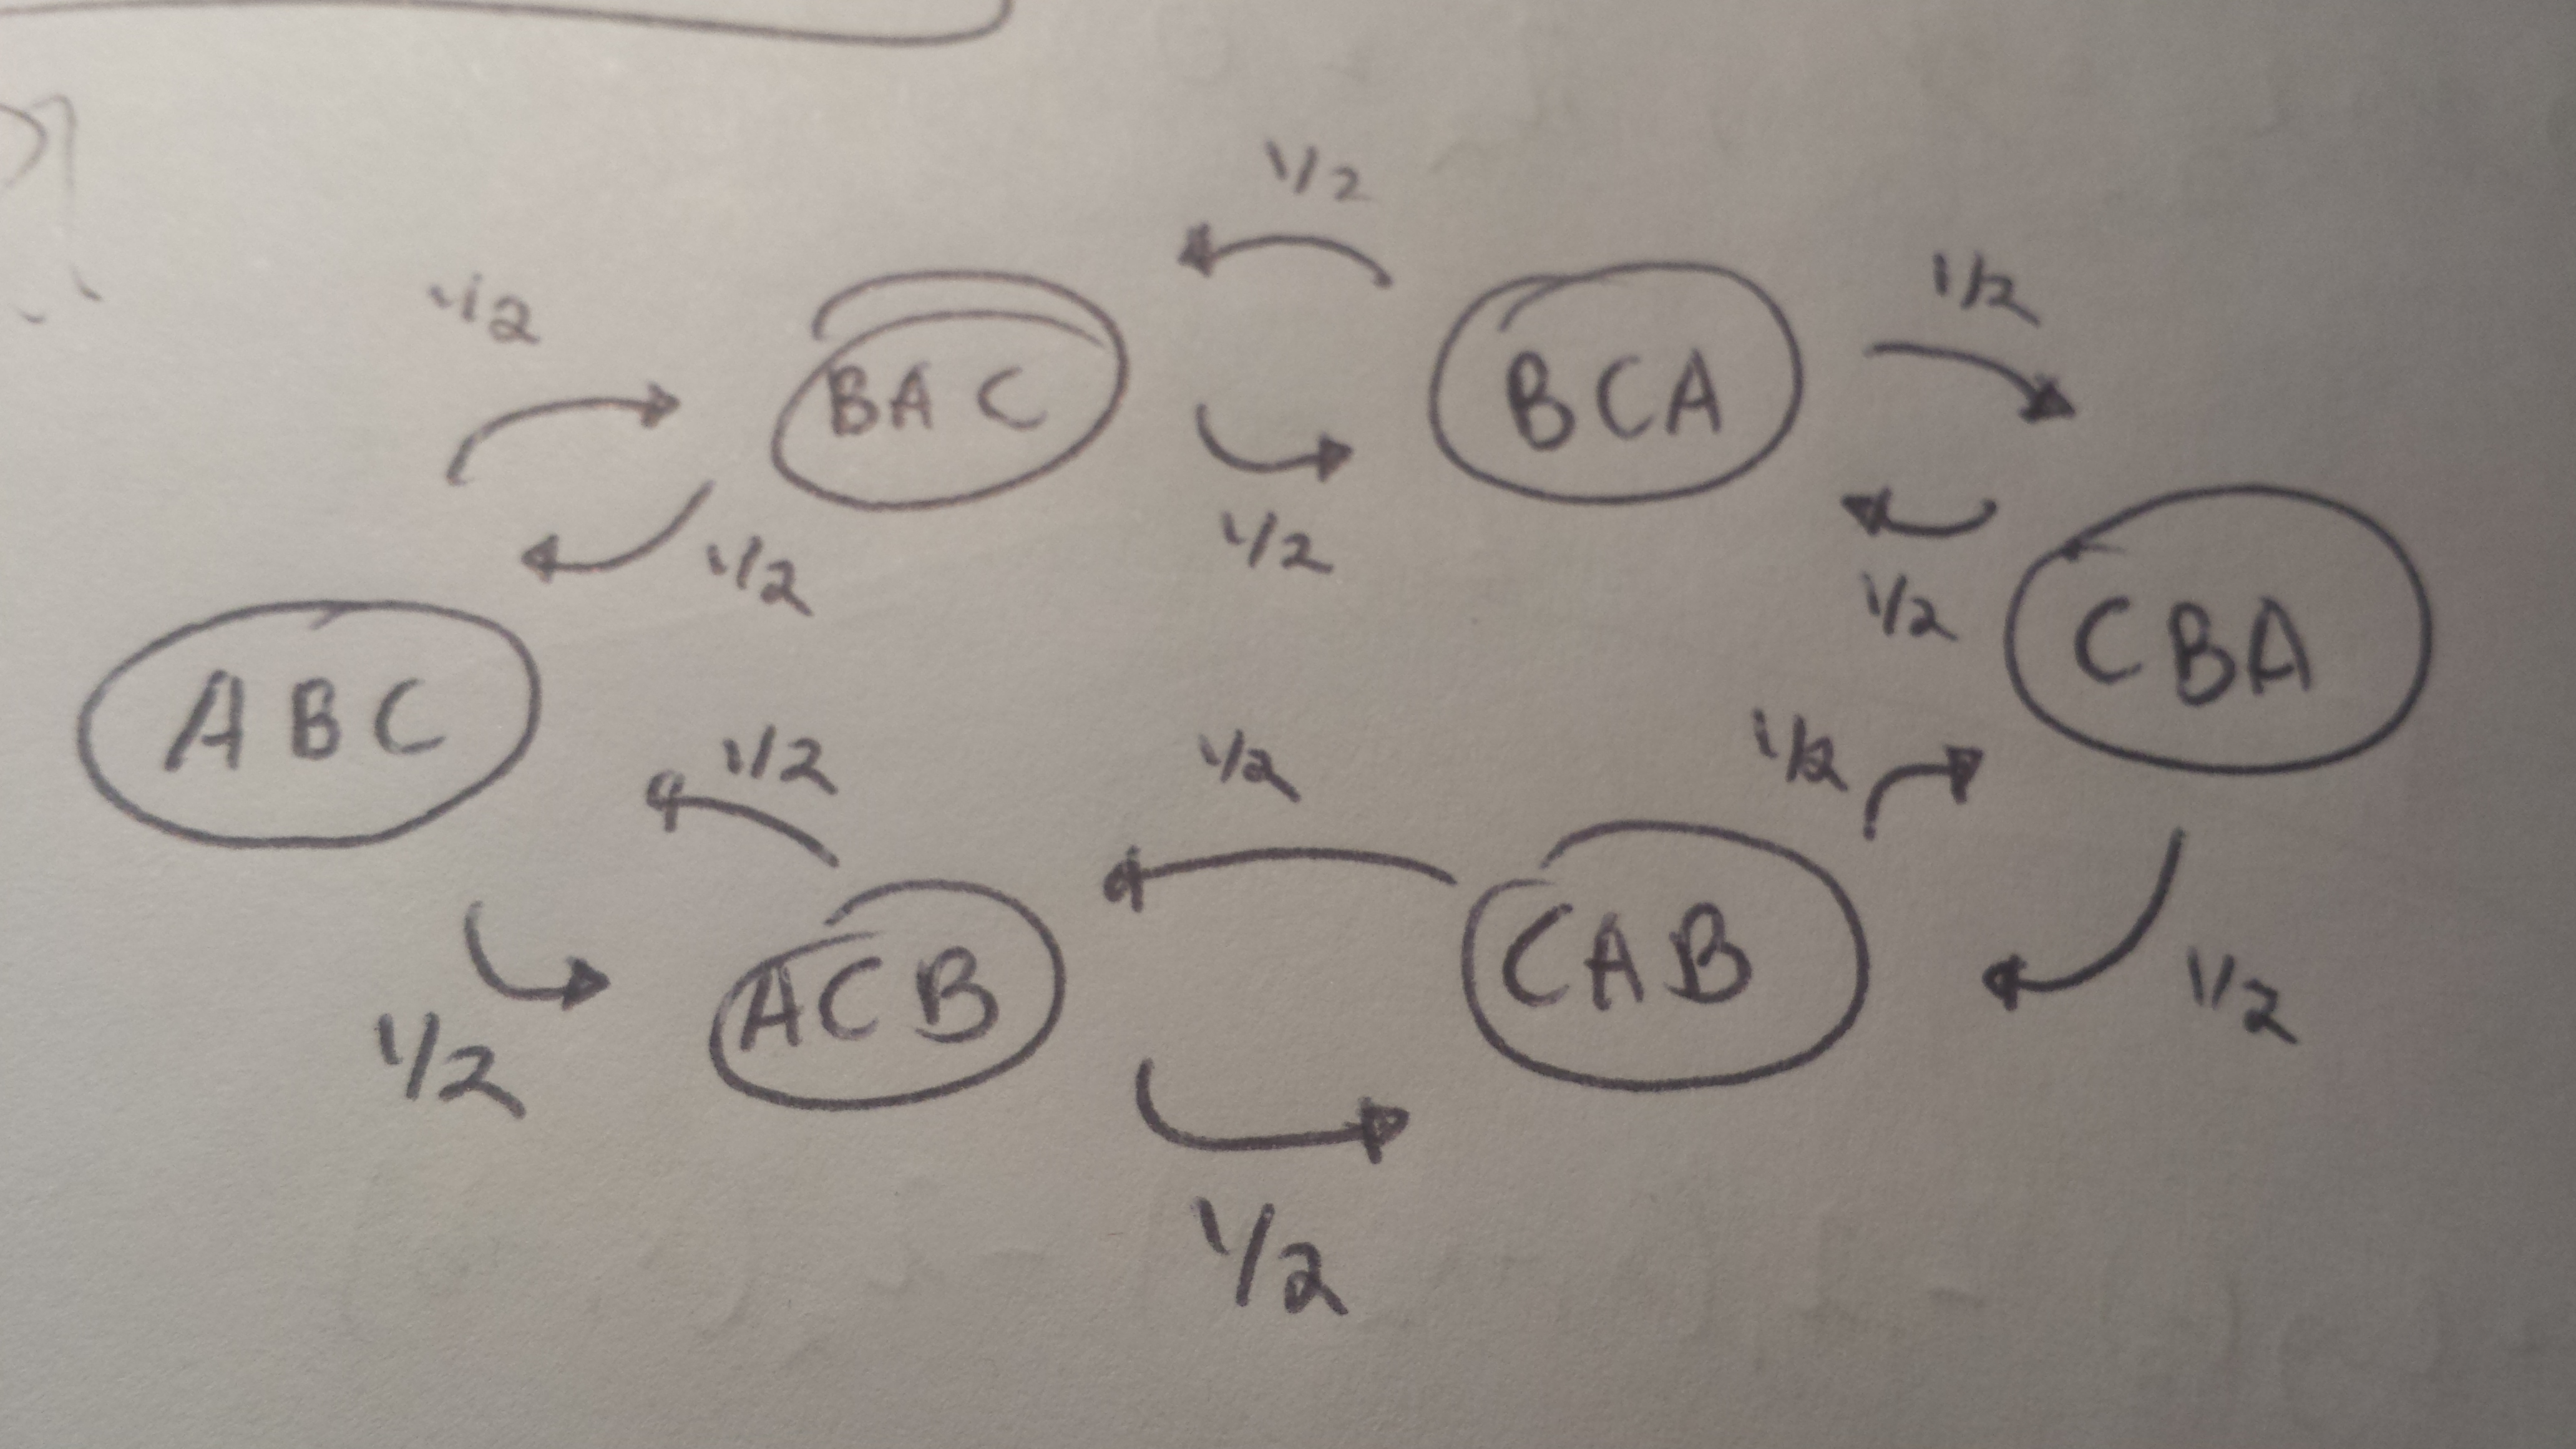
\includegraphics[width=1\textwidth]{img}
              \item [(ii)]
                Let $f(XYZ)$ be the expected number of shuffles until $CBA$ from $XYZ$. Then we have:
                $$f(ABC) = \frac{1}{2}f(BAC) + \frac{1}{2}f(ACB) + 1$$
                $$f(BAC) = \frac{1}{2}f(ABC) + \frac{1}{2}f(BCA) + 1$$
                $$f(ACB) = \frac{1}{2}f(ABC) + \frac{1}{2}f(CAB) + 1$$
                $$f(BCA) = \frac{1}{2}f(BAC) + \frac{1}{2}f(CBA) + 1$$
                $$f(CAB) = \frac{1}{2}f(ACB) + \frac{1}{2}f(CBA) + 1$$
            \end{enumerate}
          \item [(e)]
            It is \textbf{not} a Markov chain! Say $P_1(2,2) = 0, P_1(1,2) = 0.5, P_1(2,3) = 0.5, P_2(2,2) = 0.5, P_2(2,3) = 0$. Then, $P(X_2 = 3 | X_1 = 2, X_0 = 1) = P(\text{heads}) * 0.5 * 0.5 * (0.5)^3$, and $P(X_2 = 3 | X_1 = 2, X_0 = 2) = P(\text{tails}) * 0 = 0$.
        \end{enumerate}
      \item [2.]
        We have a CTMC, with $X = \{0,1,2,3,4\}$, and the rate of increasing by one is $1$, and the rate of decreasing by one is $2$. So from flow conservation we have:
        $$\pi(0) = 2 \pi(1), \pi(1) = 2 \pi(2), \cdots$$
        To solve, we know the sum of $\pi$ must be $1$, so we have:
        $$\pi(0) + \frac{1}{2} \pi(0) + \frac{1}{4} \pi(0) + \frac{1}{8} \pi(0) + \frac{1}{16} \pi(0) = 1$$
        So $\pi(0) = \frac{16}{31}, \cdots$. Since the average wait time for a taxi is $\frac{1}{2}$ a minute, and conditioning on the fact that there are $\leq 3$ other people, expected waiting time is:
        $$=\frac{\pi(0)}{\pi(0) + \pi(1) + \pi(2) + \pi(3)}(\frac{1}{2}) + \frac{\pi(1)}{\pi(0) + \pi(1) + \pi(2) + \pi(3)}(1)$$
        $$+ \frac{\pi(2)}{\pi(0) + \pi(1) + \pi(2) + \pi(3)}(\frac{3}{2}) + \frac{\pi(3)}{\pi(0) + \pi(1) + \pi(2) + \pi(3)}(2)$$
        $$=\frac{13}{15} \text{ minutes}$$
      \item [3.]
        \begin{enumerate}
          \item [(a)] 
            Let $X$ be the binomial variable denoting how many liberal votes are cast. From Chebyshev, we have:
            $$P(\abs{X - 25} \geq 25) \leq \frac{100(1/4)(3/4)}{25^2}$$
            $$P(X \geq 50) \leq \frac{3}{100}$$
        \end{enumerate}
      \item [4.]
        \begin{enumerate}
          \item [(a)]
            Since the interarrival times are Poisson, and the merging of Poisson processes is itself a Poisson process, we have that it is a Poisson process with parameter $2 \lambda t= 2t$.
          \item [(b)]
            $$P(N_1(200) = X | N_1(200) + N_2(200) = 500) = \frac{P(N_2(200) = 500-x)}{P(N_1(200) + N_2(200) = 500)}$$
            And this can be calculated from the distribution above.
          \item [(c)]
            Since the minimum of two exponentially distributd variables is exponentially distributed with combined rate, we know that this joint task will be a Poisson random variable with a combined rate of $2 \lambda t= 2t$.
          \item [(d)]
            Because of symmetry, the limit should just be $1$.
        \end{enumerate}
    \end{enumerate}
  \item The random variable $X$ is exponentially distributed with mean $1$. Given $X$, the random variable $Y$ is exponentially distributed with rate $X$.
    \begin{enumerate}
      \item Find $MLE[X|Y]$.\\\\

        MLE should just be $\argmax_x P(X=x|Y=y) = \argmax_x P(Y=y|X=x)$, since all priors are equall likely. So we have:
        $$\argmax_x xe^{-xy}$$
        =$$\argmax_x \ln(x) - xy$$
        Taking the partial derivative we get:
        $$\frac{\partial}{\partial x} \ln(x) - xy = \frac{1}{x} - y$$
        Settng it to $0$ and solving for $x$, we have:
        $$\frac{1}{x} - y = 0 \implies x = \frac{1}{y}$$
      \item Find $MAP[X|Y]$.\\\\

        Again, we have $\argmax_x P(X=x|Y=y) = \argmax_x P(Y=y|X=x)P(X=x)$. Plugging in the actual distributions, we get:
        $$=\argmax_x e^{-x}(xe^{-xy})$$
        $$=\argmax_x \ln(x) - x(y+1)$$
        Taking the partial derivative and setting to $0$, we have:
        $$\frac{\partial}{\partial x} \ln(x) - x(y+1) = 0$$
        $$\frac{1}{x} - y - 1 = 0$$
        $$x = \frac{1}{y+1}$$
    \end{enumerate}

  \item The stochastic block model (SBM) as defined in Lab 9 is a random graph $G(n,p,q)$ consisting of two communities of size $\frac{n}{2}$ each such that the probability an edge exists between two nodes of the same community is $p$ and the probability an edge exists between two nodes in different communities is $q$, where $p > q$. The goal of the problem is to exactly determine the two communities given only the graph. Show that the MAP-decision rule is equivalent to finding the min-bisection of the graph.\\\\

    Since all clusters of $\frac{n}{2}$ nodes are equally likely, since we don't really have a prior, the MAP-decision is equivalent to the MLE-decision. The MLE decision is given by:
    $$\text{MLE[two clusters given graph]} = \argmax_{\text{two clusters}} P(\text{graph given two clusters})$$
    The likelihood that a graph was generated by the two given communities is a function of the number of internal connections within a community, as well as the number of connections between the two communities. Since we're finding the maximum probability, we know that this is found by the two exclusive clusters with the maximium number of internal nodes. So we have:
    $$\argmax_{\text{two clusters}} \text{ of the number of internal edges within the clusters}$$
    Since we're maximizing the number of internal edges, and the number of edges is a constant within the graph, this is the same as minimizing the number of cross-community edges. So thus, the problem reduces to the min-bisection problem of a graph.
  \item In this problem, we use similar settings which were considered in HW2. Consider a random bipartite graph, $G_1$, with $K$ left nodes, and $M$ right nodes. Each of the $KM$ possible edges of this graph is connected with probability $p$ independently. In the following problems, we consider the situations when $M$ and $K$ are large and $Mp$ and $Kp$ are constants. Hint : Use the Poisson distribution to approximate binomial distribution and apply law of large numbers.
    \begin{enumerate}
      \item A singleton is a right node of degree one. As $M$ and $K$ get large, how many left nodes are connected to right nodes which are singletons?\\\\
        $X_i = 1$ with probability $M(p(1-p)^{K-1})$ and $= 0$ with probability $1 - M(p(1-p)^{K-1})$, as discussed in HW2. So we want to estimate:
        $$X = \sum_{i=1}^K X_i$$
        We know from the Poisson approximation of the Binomial distribution for a large $K$, that this $X$ is approaches a Poisson distribution in the limit. Similarly, from the Law of Large Numbers, we know that we approach $\mu$, which is just $np$. Thus, we have:
        $$X \approx KMp(1-p)^{K-1}$$
      \item A doubleton is a right node of degree two. As $M$ and $K$ get large, how many doubletons do we have?\\\\

        Again, we have $X_i = 1$ with probability $\binom{K}{2} p^2 (1-p)^{K-2}$. And the sum $X = \sum_{i=1}^M X_i \approx$ Poisson$(\frac{1}{2}MK(K-1)^2(1-p)^{K-2})$. And from the law of large numbers, we know that $X$ approaches $\mu$, which is:
        $$X \approx \frac{1}{2}MK(K-1)^2(1-p)^{K-2}$$
      \item We call 2 doubletons distinct, if they are not connected to the same 2 left nodes. As $K$ and $M$ get large, what is the probability that two doubletons are distinct?
    \end{enumerate}
\end{enumerate}

\end{document}
